\documentclass[11pt]{article}

\usepackage[margin=0.7in]{geometry}
\usepackage{setspace}
\usepackage{amsmath}
\usepackage{booktabs,tabularx,array}
\usepackage{xcolor}
\usepackage{microtype}
\usepackage{float}
\usepackage{listings}
\usepackage{tikz}
\usetikzlibrary{arrows.meta,positioning}
\usepackage[T1]{fontenc}
\usepackage[utf8]{inputenc}
\usepackage{lmodern}
\usepackage[skip=3pt plus 1pt]{parskip}
\usepackage{hyperref}
\usepackage{longtable}
\usepackage{enumitem}
\setlist[itemize]{topsep=4pt,itemsep=2pt,leftmargin=1.4em}
\setlist[enumerate]{topsep=4pt,itemsep=2pt,leftmargin=1.6em}
\lstset{
  basicstyle=\ttfamily\small,
  frame=single,
  columns=fullflexible,
  keepspaces=true,
  showstringspaces=false,
  breaklines=true
}

\emergencystretch=1em
\newcolumntype{L}[1]{>{\raggedright\arraybackslash}p{#1}}

\begin{document}

%% --- Inline Title ---
\begingroup
\centering
\singlespacing
\rule{\textwidth}{0.8pt}\vspace{4pt}

{\Large \bfseries Assignment 3 Project Documentation}\\[4pt]
{\large Systems Programming Mini-Project}

\vspace{4pt}\rule{\textwidth}{0.8pt}
\endgroup

\setstretch{1.02}

\section{Project Overview}

Our project is a distributed machine learning training system built with a parameter-server architecture using TCP sockets. It belongs to \textbf{Category 2: Sockets}. One server process stores the current model weights, accepts worker connections, collects gradients, updates the global model, and decides when training should stop. Each worker loads a CSV shard from disk, connects to the server, registers its dataset shape, receives weights, computes a local gradient, and sends it back.

The interaction is command-line based. The user starts the server, which creates a listening socket via \texttt{set\_up\_server\_socket()} (\texttt{net\_utils.c}, lines~21--51) and enters the \texttt{select()} loop in \texttt{main()} (\texttt{server.c}, lines~414--535). Workers are launched with a hostname and shard file; each calls \texttt{load\_data()} (\texttt{data.c}, lines~14--108), \texttt{connect\_to\_server()} (\texttt{net\_utils.c}, lines~66--103), and \texttt{send\_register()} (\texttt{worker.c}, lines~20--40), then enters its receive loop.

The machine learning component is logistic regression, implemented by \texttt{sigmoid()} (\texttt{model.c}, line~5), \texttt{compute\_gradient()} (\texttt{model.c}, line~16), \texttt{update\_weights()} (\texttt{model.c}, line~47), and \texttt{init\_weights()} (\texttt{model.c}, line~55). The main systems-programming challenges are reliable socket communication, length-prefixed message framing, partial-read handling, concurrency through \texttt{select()}, per-worker state tracking, and robust error handling.

The protocol uses four message types defined in \texttt{protocol.h} (lines~7--10): \texttt{MSG\_REGISTER}, \texttt{MSG\_WEIGHTS}, \texttt{MSG\_GRADIENT}, and \texttt{MSG\_DONE}. Together they implement a full training workflow: register, distribute weights, collect gradients, and broadcast the final model.

\section{Build Instructions}

The Makefile defines:
\begin{itemize}
    \item \texttt{PORT = 4242} (\texttt{Makefile}, line~1)
    \item \texttt{FLAGS = -Wall -Wextra -g -DPORT=\$(PORT)} (\texttt{Makefile}, line~2)
\end{itemize}

The default build target is:
\begin{lstlisting}
all: server worker gen_data
\end{lstlisting}
as defined in \texttt{Makefile} (line~4). Therefore, running \texttt{make} produces three executables:
\begin{itemize}
    \item \texttt{server}
    \item \texttt{worker}
    \item \texttt{gen\_data}
\end{itemize}

\subsection*{Build}

\begin{lstlisting}
make
\end{lstlisting}

\subsection*{Generate test shards}

\begin{lstlisting}
./gen_data <num_features> <total_samples> <num_shards>
\end{lstlisting}

For example, \texttt{./gen\_data 3 1000 4} generates \texttt{shard\_0.csv} through \texttt{shard\_3.csv}. The generator is implemented in \texttt{main()} (\texttt{gen\_data.c}, lines~13--79).

\subsection*{Run the server}

\begin{lstlisting}
./server
./server 3
\end{lstlisting}

The optional argument specifies the expected number of workers (default~1). Argument parsing is in \texttt{main()} (\texttt{server.c}, lines~381--384).

\subsection*{Run workers}

\begin{lstlisting}
./worker <server-host> <shard_file>
\end{lstlisting}

For example: \texttt{./worker localhost shard\_0.csv}. The worker parses these arguments in \texttt{main()} (\texttt{worker.c}, lines~190--197).

\subsection*{Input files}

Each shard is a CSV file where each line has the form \texttt{feature1,feature2,\ldots,featureN,label}. The final column is the binary label and the preceding columns are floating-point features. The shard-loading logic is in \texttt{load\_data()} (\texttt{data.c}, lines~14--108).

\subsection*{Cleanup}

\begin{lstlisting}
make clean
\end{lstlisting}

The cleanup rule is defined in \texttt{Makefile} (lines~36--37) and removes \texttt{*.o}, \texttt{server}, \texttt{worker}, and \texttt{gen\_data}.


\section{Architecture Diagram}

Figure~\ref{fig:arch} shows the overall structure. The server accepts connections via \texttt{accept\_connection()} (\texttt{net\_utils.c}, lines~54--63) and monitors them in its \texttt{select()} loop (\texttt{server.c}, lines~414--535). Each worker connects via \texttt{connect\_to\_server()} (\texttt{net\_utils.c}, lines~66--103) and enters its own receive loop (\texttt{worker.c}, lines~239--301). Worker-to-server traffic consists of registration and gradient messages; server-to-worker traffic consists of weight broadcasts and the termination message.

\begin{figure}[H]
\centering
\resizebox{0.92\textwidth}{!}{%
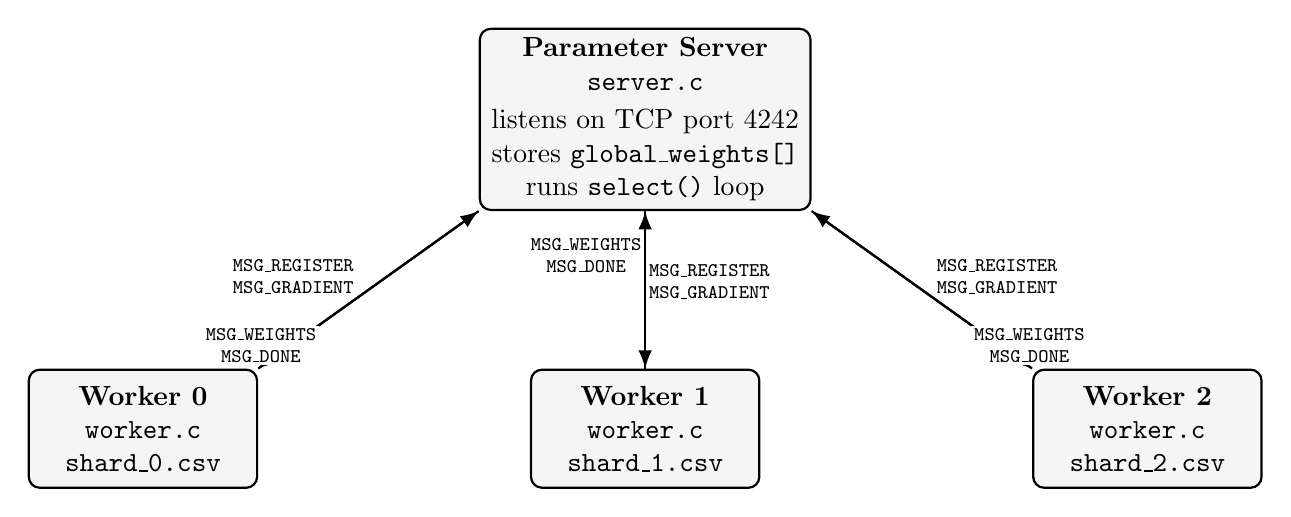
\begin{tikzpicture}[
    node distance=1.6cm and 2.3cm,
    proc/.style={
        draw,
        rounded corners,
        align=center,
        minimum width=2.9cm,
        minimum height=1.5cm,
        fill=gray!8
    },
    serv/.style={
        draw,
        rounded corners,
        align=center,
        minimum width=4.2cm,
        minimum height=1.9cm,
        fill=gray!8
    },
    msg/.style={
        font=\scriptsize,
        align=center,
        fill=white,
        inner sep=1pt
    },
    ->, >=Latex, thick
]

\node[serv] (server) {
\textbf{Parameter Server}\\
\texttt{server.c}\\[2pt]
listens on TCP port 4242\\
stores \texttt{global\_weights[]}\\
runs \texttt{select()} loop
};

\node[proc, below left=2.0cm and 2.8cm of server] (w0) {
\textbf{Worker 0}\\
\texttt{worker.c}\\
\texttt{shard\_0.csv}
};

\node[proc, below=2.0cm of server] (w1) {
\textbf{Worker 1}\\
\texttt{worker.c}\\
\texttt{shard\_1.csv}
};

\node[proc, below right=2.0cm and 2.8cm of server] (w2) {
\textbf{Worker 2}\\
\texttt{worker.c}\\
\texttt{shard\_2.csv}
};

\draw[->] (w0.north east) -- (server.south west)
    node[pos=0.45, above left, msg] {\texttt{MSG\_REGISTER}\\\texttt{MSG\_GRADIENT}};
\draw[->] (w1.north) -- (server.south)
    node[pos=0.55, right, msg] {\texttt{MSG\_REGISTER}\\\texttt{MSG\_GRADIENT}};
\draw[->] (w2.north west) -- (server.south east)
    node[pos=0.45, above right, msg] {\texttt{MSG\_REGISTER}\\\texttt{MSG\_GRADIENT}};

\draw[->] (server.south west) -- (w0.north east)
    node[pos=0.72, below left, msg] {\texttt{MSG\_WEIGHTS}\\\texttt{MSG\_DONE}};
\draw[->] (server.south) -- (w1.north)
    node[pos=0.28, left, msg] {\texttt{MSG\_WEIGHTS}\\\texttt{MSG\_DONE}};
\draw[->] (server.south east) -- (w2.north west)
    node[pos=0.72, below right, msg] {\texttt{MSG\_WEIGHTS}\\\texttt{MSG\_DONE}};

\end{tikzpicture}%
}
\caption{Overall system architecture.}
\label{fig:arch}
\end{figure}

\section{Communication Protocol}
\label{sec:protocol}

\subsection{Common Framing and Header Format}

All messages share a common wire format: a 5-byte header followed by a
variable-length payload. The header consists of a 1-byte message type code at
offset~0, followed by a 4-byte payload size in network byte order (big-endian)
at offsets~1--4. Multi-byte integers in the payload are also in network byte
order, converted with \texttt{htonl}/\texttt{ntohl}. Floats are transmitted in
host byte order; since both server and workers run on teach.cs (x86-64), no
float byte-swapping is needed.

A shared helper function in \texttt{io\_utils} handles header serialization:
\texttt{send\_header(int fd, uint8\_t type, uint32\_t payload\_len)}
constructs a 5-byte buffer. Byte~0 is the type code, and bytes~1--4 are
\texttt{htonl(payload\_len)}. It sends the buffer via \texttt{write\_all()}.
Returns~0 on success, $-1$ on failure.
(\texttt{io\_utils.c}, line~77)
On the receiving side, header parsing is done inline: the receiver reads
byte~0 as the type code, copies bytes~1--4 into a \texttt{uint32\_t}, and
converts with \texttt{ntohl} to obtain the host-order payload length.

\subsubsection*{Header byte layout (all messages)}

\begin{table}[H]
\centering
\begin{tabular}{@{}c c l l@{}}
\toprule
\textbf{Offset} & \textbf{Size (bytes)} & \textbf{Field} & \textbf{Encoding} \\
\midrule
0 & 1 & \texttt{type} & Message type code (\texttt{0x01}--\texttt{0x04}) \\
1 & 4 & \texttt{payload\_len} & \texttt{htonl(payload\_len)}; payload size in bytes \\
\bottomrule
\end{tabular}
\end{table}

On the worker side, complete blocking reads are handled by \texttt{read\_all()} (io\_utils.c, lines 13--23). On the server side, partial nonblocking message assembly is handled by \texttt{accumulate\_read()} (io\_utils.c, lines 48--71). This structure avoids ambiguity in message boundaries and allows the server to handle fragmented TCP input safely.

\subsection{MSG\_REGISTER (0x01)}

\textbf{Direction:} Worker $\to$ Server, sent once immediately after connecting.
\textbf{Total message size:} $5 + 8 = 13$~bytes.

\subsubsection*{Byte layout}

\begin{table}[H]
\centering
\begin{tabular}{@{}c c l l@{}}
\toprule
\textbf{Offset} & \textbf{Size} & \textbf{Field} & \textbf{Encoding} \\
\midrule
0 & 1 & \texttt{type} & \texttt{0x01} (\texttt{MSG\_REGISTER}) \\
1 & 4 & \texttt{payload\_len} & \texttt{htonl(8)} \\
5 & 4 & \texttt{num\_features} & \texttt{htonl(num\_features)} \\
9 & 4 & \texttt{num\_samples} & \texttt{htonl(num\_samples)} \\
\bottomrule
\end{tabular}
\end{table}

\textbf{Semantics.}
\texttt{send\_register()} (worker.c, lines 20--40) serializes both fields with \texttt{htonl()} and sends the message with \texttt{write\_all()}.

On the server side, \texttt{dispatch\_message()} (server.c, lines 337--369) routes the message to \texttt{handle\_register()} (server.c, lines 287--327), which deserializes and validates the feature and sample counts, stores them in the \texttt{worker\_info} slot, and sets the worker's state to registered (state~1). If this is the first worker, the server also initializes the global weights with \texttt{init\_weights()} (model.c, lines 55--60). The server does not broadcast weights immediately; training starts later in \texttt{main()} (server.c, lines 485--501) once enough workers have registered.

\subsubsection*{Error handling}

\begin{itemize}
  \item If the worker sends an invalid feature count, \texttt{handle\_register()} (\texttt{server.c}, lines~300--304) logs an error and disconnects the worker through \texttt{handle\_disconnect()} (\texttt{server.c}, lines~278--285).
  \item If the worker sends a nonpositive sample count, \texttt{handle\_register()} (\texttt{server.c}, lines~316--320) logs an error and disconnects the worker.
  \item If a later worker's feature count does not match the server's established feature count, \texttt{handle\_register()} (\texttt{server.c}, lines~309--314) disconnects that worker.
\end{itemize}

\subsection{MSG\_WEIGHTS (0x02)}

\textbf{Direction:} Server $\to$ Worker, sent at the start of each round (first broadcast after enough workers register).
\textbf{Total message size:} $5 + 8 + n \times 4$~bytes, where $n$ is the number of features.

\subsubsection*{Byte layout}

\begin{table}[H]
\centering
\begin{tabular}{@{}c c l l@{}}
\toprule
\textbf{Offset} & \textbf{Size} & \textbf{Field} & \textbf{Encoding} \\
\midrule
0  & 1            & \texttt{type}          & \texttt{0x02} (\texttt{MSG\_WEIGHTS}) \\
1  & 4            & \texttt{payload\_len}  & \texttt{htonl(8 + n * sizeof(float))} \\
5  & 4            & \texttt{round}         & \texttt{htonl(round)} \\
9  & 4            & \texttt{num\_features} & \texttt{htonl(n)} \\
13 & $n \times 4$ & \texttt{weights}       & \texttt{float[n]}, host byte order \\
\bottomrule
\end{tabular}
\end{table}

\subsubsection*{Semantics}

\texttt{send\_weights\_to\_worker()} (\texttt{server.c}, lines~46--78) constructs the message in a stack buffer and sends it with \texttt{write\_all()}, advancing the worker's state and resetting \texttt{gradient\_received}. The server broadcasts to all registered workers through \texttt{broadcast\_weights()} (\texttt{server.c}, lines~85--95). On the worker side, the main receive loop (\texttt{worker.c}, lines~239--301) reads each header with \texttt{read\_all()} and dispatches by type. For \texttt{MSG\_WEIGHTS} (lines~250--285), it validates the payload size, reads the payload with \texttt{read\_all()}, deserializes round and feature count with \texttt{ntohl}, and copies the weights into local memory.

\subsubsection*{Error handling}

\begin{itemize}
  \item If the payload size is too small (fewer than 8~bytes), the worker logs an error, drains the remaining payload bytes, and continues to the next message (\texttt{worker.c}, lines~251--258). If the payload exceeds the local buffer size, the worker logs an error and exits the receive loop (\texttt{worker.c}, lines~260--263).
  \item If the received feature count exceeds the shard's feature count, the worker truncates to the shard's value (\texttt{worker.c}, line~272).
  \item If a broadcast send fails on the server side, \texttt{broadcast\_weights()} disconnects the affected worker through \texttt{handle\_disconnect()} (\texttt{server.c}, lines~278--285).
\end{itemize}

\subsection{MSG\_GRADIENT (0x03)}

\textbf{Direction:} Worker $\to$ Server, sent once per round after computing the local gradient.
\textbf{Total message size:} $5 + 12 + n \times 4$~bytes.

\subsubsection*{Byte layout}

\begin{table}[H]
\centering
\begin{tabular}{@{}c c l l@{}}
\toprule
\textbf{Offset} & \textbf{Size} & \textbf{Field} & \textbf{Encoding} \\
\midrule
0  & 1             & \texttt{type}         & \texttt{0x03} (\texttt{MSG\_GRADIENT}) \\
1  & 4             & \texttt{payload\_len} & \texttt{htonl(12 + n * sizeof(float))} \\
5  & 4             & \texttt{round}        & \texttt{htonl(round)}; current training round \\
9  & 4             & \texttt{num\_features} & \texttt{htonl(n)} \\
13 & 4             & \texttt{local\_loss}  & \texttt{float}, host byte order; average loss on this worker's shard \\
17 & $n \times 4$  & \texttt{gradients}    & \texttt{float[n]}, host byte order; gradient vector \\
\bottomrule
\end{tabular}
\end{table}

\subsubsection*{Semantics}
Once \texttt{accumulate\_read()} assembles a complete message,
\texttt{dispatch\_message()} (\texttt{server.c}, line~337) routes it to
\texttt{handle\_gradient()} (\texttt{server.c}, line~123), which deserializes
each field with \texttt{memcpy}/\texttt{ntohl}, validates
\texttt{num\_features} against \texttt{MAX\_FEATURES} (lines~138--142) and
\texttt{round} against \texttt{current\_round} (line~150), then stores the
gradient and sets \texttt{gradient\_received = 1} (lines~157--159). On
validation failure it returns $-1$; the caller logs a warning but does not
disconnect the worker. The gradient barrier and aggregation logic are described
in Section~\ref{sec:concurrency}.

On the worker side, \texttt{send\_gradient()} (\texttt{worker.c}, line~116)
serializes the payload with \texttt{memcpy}/\texttt{htonl}, then sends header
and payload via \texttt{send\_header()} and \texttt{write\_all()}
(lines~140--141).

\subsubsection*{Error handling}

\begin{itemize}
  \item If \texttt{num\_features} is out of range (zero, negative, or exceeds
    \texttt{MAX\_FEATURES}), \texttt{handle\_gradient()} prints a diagnostic to
    stderr and returns $-1$ without copying any gradient data. The worker's
    \texttt{gradient\_received} remains~0, so the malformed gradient is not
    counted toward aggregation. This prevents a buffer overflow on
    \texttt{w->gradients}.
  \item If \texttt{round} does not match \texttt{current\_round}, the gradient
    is stale. The server logs a warning to stderr
    (\texttt{"Stale gradient: got round \%d, expected \%d"}) and returns $-1$
    without modifying any state. This can happen if a worker was slow and is
    still sending a gradient from a previous round's weights.
  \item If \texttt{write\_all()} fails on the worker side (returns $-1$),
    \texttt{send\_gradient()} prints an error to stderr and returns $-1$. The
    caller treats this as a server disconnect, closes the socket, and exits.
  \item If the worker disconnects before sending its gradient,
    \texttt{accumulate\_read()} returns $-1$ and the server cleans up the worker
    via \texttt{handle\_disconnect()}. The remaining active workers' gradients
    are still collected normally.
\end{itemize}

\subsection{MSG\_DONE (0x04)}

\textbf{Direction:} Server $\to$ all active workers, sent exactly once when
\texttt{check\_termination()} (\texttt{server.c}, line~229) returns~1
(global loss below \texttt{LOSS\_THRESHOLD}~(0.001) or \texttt{current\_round}
reaches \texttt{MAX\_ROUNDS}~(100)).
\textbf{Total message size:} $5 + 8 + n \times 4$~bytes.

\subsubsection*{Byte layout}

\begin{table}[H]
\centering
\begin{tabular}{@{}c c l l@{}}
\toprule
\textbf{Offset} & \textbf{Size} & \textbf{Field} & \textbf{Encoding} \\
\midrule
0  & 1             & \texttt{type}         & \texttt{0x04} (\texttt{MSG\_DONE}) \\
1  & 4             & \texttt{payload\_len} & \texttt{htonl(8 + n * sizeof(float))} \\
5  & 4             & \texttt{num\_features} & \texttt{htonl(n)} \\
9  & 4             & \texttt{final\_loss}  & \texttt{float}, host byte order; the last global loss value \\
13 & $n \times 4$  & \texttt{weights}      & \texttt{float[n]}, host byte order; the final trained model \\
\bottomrule
\end{tabular}
\end{table}

\subsubsection*{Semantics}
On the server side, \texttt{broadcast\_done()} (\texttt{server.c}, line~241)
builds the payload once, then for each active worker
(\texttt{fd != -1}, \texttt{state == 2}) sends the header via
\texttt{send\_header()} and the payload via \texttt{write\_all()}
(lines~262--263). On the worker side, when the main receive loop
(\texttt{worker.c}, line~239) reads a header with type \texttt{MSG\_DONE},
\texttt{handle\_done()} (\texttt{worker.c}, line~153) reads the payload with
\texttt{read\_all()} (line~159), deserializes all fields with
\texttt{memcpy}/\texttt{ntohl}, prints the final loss and weights to stdout
(lines~178--183), and returns~1. The main loop then breaks and the worker
cleans up.

\subsubsection*{Error handling}

\begin{itemize}
  \item If \texttt{write\_all()} fails for a particular worker during broadcast,
    the server logs an error to stderr and continues sending to the remaining
    workers. The function returns $-1$ to indicate that at least one send
    failed.
  \item If \texttt{read\_all()} fails on the worker side (server disconnected
    before finishing the message), \texttt{handle\_done()} prints an error to
    stderr and returns $-1$. The main loop breaks regardless and the worker
    performs its normal cleanup (closing the socket and freeing memory).
\end{itemize}

\section{Concurrency Model}
\label{sec:concurrency}

This project uses Category~2 concurrency: a single-threaded server manages
multiple worker clients through the \texttt{select()} system call. There are no
threads and no \texttt{fork()}-per-client.

\subsection{The \texttt{select()} Loop}

The server's main loop (\texttt{server.c}, line~414) follows the
\texttt{simpleselect.c} pattern. Two \texttt{fd\_set} variables are maintained:
\texttt{allset} tracks the listening socket plus every connected worker, and
\texttt{rset} is a copy passed to \texttt{select()}. Each iteration copies
\texttt{rset = allset} and resets a 10-second timeout (lines~415--419), then
calls \texttt{select(maxfd + 1, \&rset, NULL, NULL, \&tv)}. On timeout the
server logs a status message and continues; on \texttt{EINTR} it retries
(line~423).

After \texttt{select()} returns with readable descriptors, the server checks two
things in order:

\begin{enumerate}
  \item \textbf{New connections.} If \texttt{FD\_ISSET(listen\_fd, \&rset)} is
    true (line~433), the server accepts the connection with
    \texttt{accept\_connection()}, adds the new fd to \texttt{allset} with
    \texttt{FD\_SET()} (line~441), updates \texttt{maxfd} if needed (line~442),
    and initializes a \texttt{worker\_info} slot via \texttt{add\_worker()}.

  \item \textbf{Existing workers.} The server iterates over all
    \texttt{MAX\_WORKERS} slots (line~448). For each slot with a valid fd that
    is set in \texttt{rset}, it calls \texttt{accumulate\_read()} (line~450).
\end{enumerate}

\subsection{How Blocking on a Single Client Is Avoided}

The server never calls a blocking read loop for any individual client.
\texttt{accumulate\_read()} (\texttt{io\_utils.c}, line~48) performs exactly one
\texttt{read()} call (line~49), appending whatever bytes are available to that
worker's \texttt{recv\_buf}. It returns~0 if the header or payload is still
incomplete (lines~57--58,~67--68), or~1 when a full message is ready (line~70). Because
only one system call is made per worker per iteration, a slow worker does not
block service to others.

When \texttt{accumulate\_read()} returns~1, the server loops (line~470) calling
\texttt{dispatch\_message()} (line~337) to route each complete message to
\texttt{handle\_register()} or \texttt{handle\_gradient()} by type byte. After
processing, \texttt{dispatch\_message()} shifts remaining bytes forward with
\texttt{memmove()} (lines~364--368), handling the case where a single
\texttt{read()} delivered multiple messages.

When \texttt{accumulate\_read()} returns $-1$ (disconnect or error), the server
calls \texttt{handle\_disconnect()} (\texttt{server.c}, line~278) to close the
fd and reset the \texttt{worker\_info} slot. The calling code in the main loop
then removes the fd from \texttt{allset} with \texttt{FD\_CLR()} (line~457) and
recalculates \texttt{maxfd} by scanning all active workers if the disconnected
fd was the current \texttt{maxfd} (lines~459--466).

\subsection{Synchronous Gradient Barrier}

At the end of each select loop iteration, \texttt{all\_gradients\_received()}
(\texttt{server.c}, line~167) checks whether every active worker
(\texttt{fd != -1}, \texttt{state == 2}) has \texttt{gradient\_received == 1}.
If \texttt{count\_active\_workers()} (line~107)
returns~0, the function returns~0 so that aggregation does not run on an empty set. When all gradients are in,
\texttt{aggregate\_and\_update()} (line~187) computes a weighted average and
updates the model. If \texttt{check\_termination()} (line~229) returns true,
\texttt{broadcast\_done()} sends the final model; otherwise
\texttt{broadcast\_weights()} starts the next round (lines~516--532). This
barrier ensures no worker receives new weights until all active workers have
reported, without any blocking beyond the select call itself.

Workers use blocking I/O (\texttt{read\_all()} in \texttt{io\_utils.c},
line~13; \texttt{write\_all()} in \texttt{io\_utils.c}, line~29) because each
worker communicates with only one server. Both functions loop until the
requested number of bytes has been transferred or an error occurs, so the
worker never tries to parse partial headers or payloads.


\section{Error Handling and Robustness}

Both the server and worker call \texttt{signal(SIGPIPE, SIG\_IGN)} at startup
so that writes to a closed socket produce an \texttt{EPIPE} error (caught via
the \texttt{write()} return value) instead of terminating the process. On the
server side, this call is at \texttt{server.c} line~401. On the worker side,
the call is at \texttt{worker.c} line~204, in \texttt{main()} before any I/O
begins.

\subsection{Bad Behavior 1: Worker Disconnects Mid-Training}

\subsubsection*{Detection}
When the server calls \texttt{accumulate\_read()} for a worker whose connection
has been closed, \texttt{read()} returns~0 (EOF) or $-1$ (error).
\texttt{accumulate\_read()} returns $-1$ in either case (\texttt{io\_utils.c},
line~51).

\subsubsection*{Handling}
The server calls \texttt{handle\_disconnect()} (\texttt{server.c}, line~278) to
close the fd and reset the \texttt{worker\_info} slot. The main loop then
removes the fd from \texttt{allset} with \texttt{FD\_CLR()} (line~457) and
recalculates \texttt{maxfd} (lines~459--466). Since
\texttt{all\_gradients\_received()} and \texttt{aggregate\_and\_update()} only
consider workers with \texttt{fd != -1}, the disconnected worker is excluded
from both the gradient barrier and the weighted average. A guard in
\texttt{all\_gradients\_received()} (line~169) returns~0 when no workers remain,
preventing aggregation from running on an empty set. A separate check at line~503 exits the server
gracefully when all workers have disconnected.

\subsection{Bad Behavior 2: Partial Read on Gradient Message}

\subsubsection*{Detection}
TCP does not guarantee that a full application-level message arrives in a single
\texttt{read()} call. When the server calls \texttt{accumulate\_read()} and
\texttt{read()} returns fewer bytes than needed for a complete
\texttt{MSG\_GRADIENT} message, the function detects this by comparing
\texttt{recv\_len} against \texttt{HEADER\_SIZE + payload\_size}
(\texttt{io\_utils.c}, line~67).

\subsubsection*{Handling}
\texttt{accumulate\_read()} returns~0, leaving the partial data in the worker's
\texttt{recv\_buf}. The server returns to the select loop and continues
servicing other workers normally. The next time this worker's fd becomes
readable, \texttt{accumulate\_read()} appends more bytes to \texttt{recv\_buf}
at the current \texttt{recv\_len} offset (line~49). This repeats until the full
message (header + payload) is assembled, at which point
\texttt{accumulate\_read()} returns~1 and the message is dispatched. The
per-worker \texttt{recv\_buf} and \texttt{recv\_len} fields in
\texttt{struct worker\_info} (\texttt{protocol.h}, line~31) make this
possible. Each worker's partial state is tracked independently.

\subsection{Bad Behavior 3: Worker Sends Gradient for Wrong Round (Stale Gradient)}

\subsubsection*{Detection}
Each \texttt{MSG\_GRADIENT} message includes a \texttt{round} field. When
\texttt{handle\_gradient()} (\texttt{server.c}, line~123) deserializes this
field (line~129), it compares the received round against the server's
\texttt{current\_round} (line~150).

\subsubsection*{Handling}
If the rounds do not match, the gradient is stale, likely from a slow worker
that was still computing from a previous round's weights. The server prints a
warning to stderr (\texttt{"Stale gradient: got round \%d, expected \%d"}) and
returns $-1$ without modifying any state. The gradient is not counted toward the
current round's aggregation and \texttt{gradient\_received} remains~0 for that
worker. The server will wait for this worker to send a gradient with the correct
round number before proceeding.

\section{Team Contributions}

\textbf{Angela Su} was primarily responsible for the gradient-aggregation and training-loop side of the project. This included implementing the logistic-regression model functions in \texttt{model.c}, the worker-to-server \texttt{MSG\_GRADIENT} path, the server-side gradient handling and aggregation logic, the training termination condition, and the final \texttt{MSG\_DONE} broadcast.

\textbf{Jinxi Li} was primarily responsible for the connection-management and weight-broadcast side of the project, together with the networking and data-loading foundation. This included implementing the TCP helper functions in \texttt{net\_utils.c}, the CSV shard loader in \texttt{data.c}, the worker-side registration path, and the server-side worker admission, registration handling, and weight broadcast logic.


\end{document}